\documentclass{standalone}

\usepackage[usenames,dvipsnames,svgnames,table]{xcolor}
\usepackage{gastex}

\usepackage{tikz}
\def\pgfsysdriver{pgfsys-tex4ht.def}

\usetikzlibrary{arrows,automata,positioning}

\newcommand{\smaller}{\mathrm{S}}
\newcommand{\bigger}{\mathrm{B}}
\newcommand{\start}{\mathrm{start}}
\newcommand{\ed}{\mathrm{end}}


\begin{document}

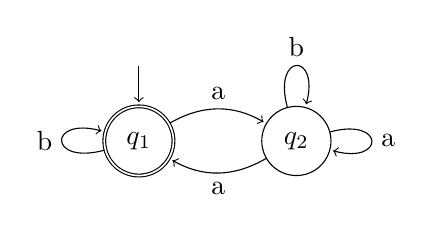
\begin{tikzpicture}[shorten >=1pt,node distance=2cm,auto]
  \tikzstyle{every state}=[draw={rgb:black,10;white,0}]
  \tikzstyle{non state}=[]

  \node[state,accepting] (q_1) []  {$q_1$};
  \node[non state] (q_0) [above=0.5cm of q_1]  {};
  \node[state]           (q_2) [right of=q_1]     {$q_2$};
  
  \path[->]
  (q_0) edge []				node {} (q_1)  
  (q_1) edge [loop left]  node {b} (  )
        edge [bend left]  node {a} (q_2)
  (q_2) edge [loop above]  node {b} (  )
  		edge [loop right]  node {a} (  )
        edge [bend left]  node {a} (q_1);
\end{tikzpicture}

\end{document}